\section{Model}
\label{sec:model}

In this section, we first formulate the machine comprehension problem and then describe the model. 

\subsection{Problem Statement}
\label{subsec:problemstatement}

The machine comprehension task considered in this paper is as follows. Given a context paragraph with $T$ words, C = \{$c_1$, $c_2$, ..., $c_T$\} and a query sentence with $J$ words, Q = \{$q_1$, $q_2$, ... $q_J$\}, output a span S = \{$c_i$, $c_{i+1}$,...${c_{i+j}}$\} from the original paragraph C that satisfactorily answers the question. Section ~\ref{subsec:metricdetails} describes two metrics that are widely used in literature for evaluating this task. We use $d$ to represent the hidden size used by several layers of the model.

\begin{table}[htbp]
    \caption{An example of a machine comprehension task.}
    \label{table:economicSchools} 
    \centering
    \begin{tabular}{|l|p{0.8\linewidth}|}
    \hline
    Question   &  Economy, Energy and Tourism is one of the what? \tabularnewline \hline
    Context  & Subject Committees are established at the beginning of each parliamentary session, and again the members on each committee reflect the balance of parties across Parliament. Typically each committee corresponds with one (or more) of the departments (or ministries) of the Scottish Government. The \textcolor{blue}{current Subject Committees} in the fourth Session are: Economy, Energy and Tourism; Education and Culture; Health and Sport; Justice; Local Government and Regeneration; Rural Affairs, Climate Change and Environment; Welfare Reform; and Infrastructure and Capital Investment \tabularnewline \hline
    Answer   & current Subject Committees \tabularnewline \hline
    \end{tabular}
 
\end{table}

\subsection{Model Overview}
\label{subsec:models}

Several state-of-the-art machine comprehension models have a similar structure. They have (a) an embedding layer (b) an embedding encoder layer (c) an attention flow layer (d) a model encoder layer and (e) an output layer. 

We introduce two novel extensions to this structure.  One, we add a Embedding Attention Layer between the input Embedding Layer and the Embedding Encoder Layer, with the goal of introducing early attention in the modeling process. Second, for the Embedding Encoder Layer we use a combination of recurrent and convolution operations to make it rich with both sequential and local interactions. Our machine comprehension model is thus a hierarchical multi-stage process consisting of six layers. 

\begin{enumerate}
\item Embedding Layer. 
\item Embedding Attention Layer.
\item Embedding Encoder Layer.
\item Attention Flow Layer.
\item Model Encoder Layer.
\item Output Layer.
\end{enumerate}

\begin{figure*}[h!]
\centering
	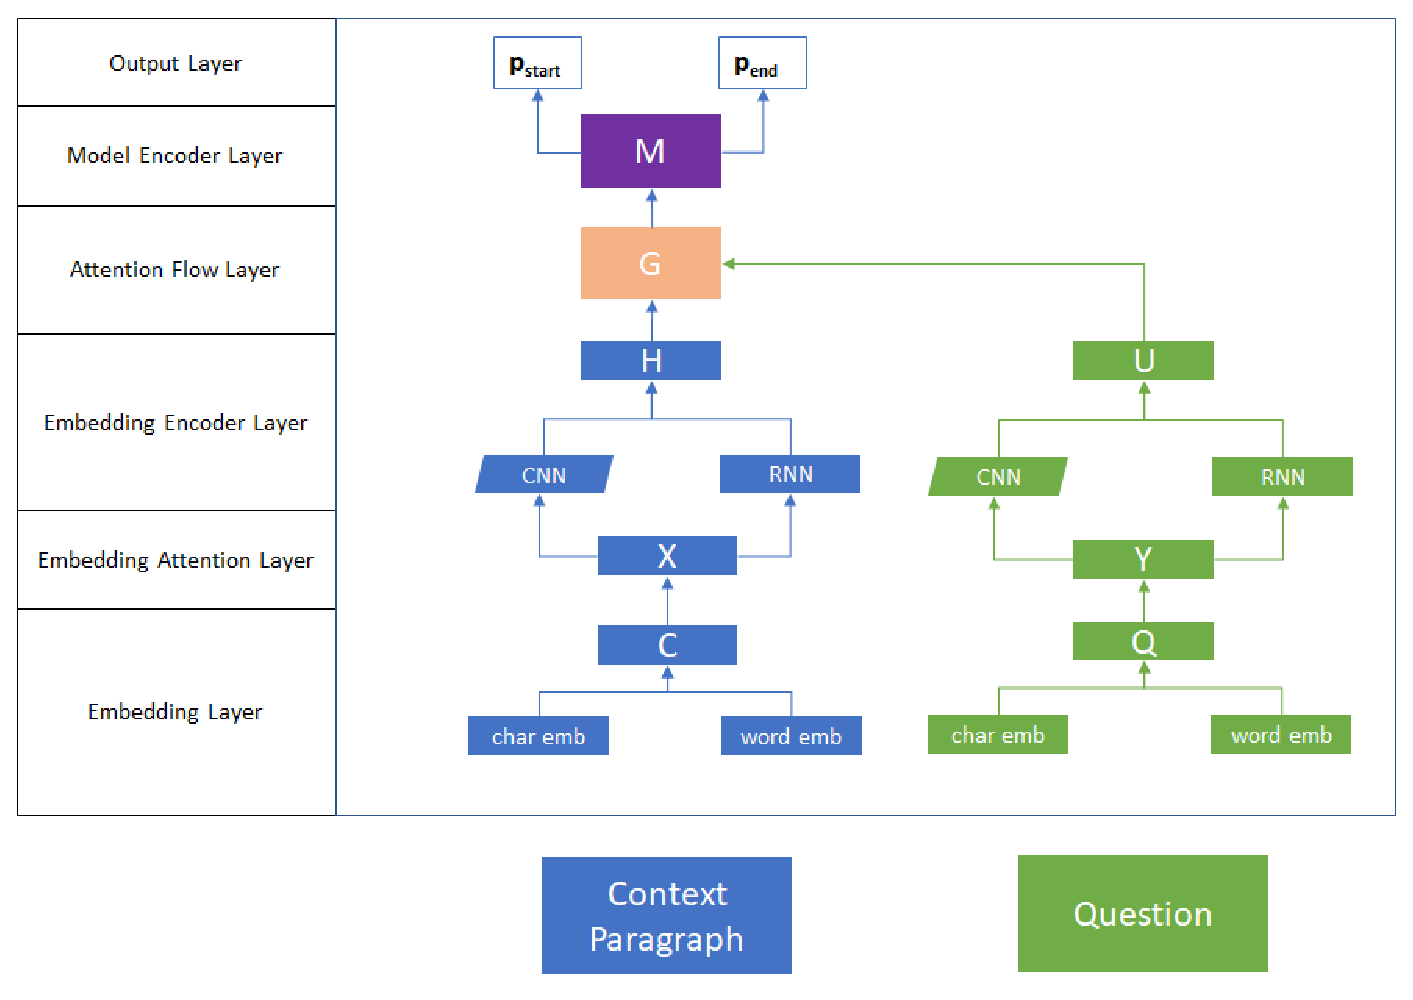
\includegraphics[width=12cm]{Figs4Paper/Model2.eps}
  \caption{Model architecture}
  \label{fig:modelarchitecture}
\end{figure*}

The details of each of the layers are as follows.

\paragraph{1. Embedding Layer.} In this layer we mix character embeddings with word embeddings. 

For character embeddings, we use a method similar to that proposed by Kim et al \cite{kim2016character}. We first convert a word to its character indices. We then pad (or truncate) each word so it has length $m_{word}$.  For each of these characters we lookup a dense character embedding (which has shape ${e_{char}}$). To combine the character embeddings, we use 1-dimensional convolutions over $m_{word}$ using ${e_{char}}$ as the input channel size and ${e_{word}}$ as the output channel size. The output of the CNN are max-pooled over the entire width to obtain a fixed-size vector of shape ${e_{word}}$ for each word. 

For word embeddings, we use pre-trained word vectors from GloVe \cite{pennington2014glove} to obtain the fixed embedding for each word. The size of the word embeddings is ${e_{word}}$ which is the same as the shape of the character-level embeddings for each word.  

The concatenation of the character and word embeddings is passed to a Highway Network \cite{srivastava2015highway}. We do this for both the context sentence $C$ and also the question $Q$. So now we have two matrices \textbf{C} $\in \mathbb{R}^{T, d}$  and \textbf{Q} $\in \mathbb{R}^{J, d}$ corresponding to the context and question respectively.

\paragraph{2. Embedding Attention Layer.} The motivation for adding this layer is to attend to the embeddings provided by the previous layer. This layer starts early attention to the word and character character embeddings. As before, we do this for both the context sentence $C$ and also the question $Q$ , and concatenate the results with the embedding layer output giving us two matrices \textbf{X} $\in \mathbb{R}^{T, 2d}$  and \textbf{Y} $\in \mathbb{R}^{J, 2d}$ corresponding to the context and question respectively. 

\paragraph{3. Embedding Encoder Layer.} The purpose of this layer is to encode the relationships between the embeddings provided by the previous layers. On one hand we want to model the temporal interactions between words. For this we use a bi-directional LSTM. This results in two matrices of shape $(T, 2d)$ and $(J, 2d)$ corresponding to the context and question respectively. 

We also model local interactions between the embeddings output by the embedding attention layer. We use 1-dimensional convolutions over the sequence length using $2d$ as both the input and output  channel size. We do this using a kernel size 1,  which results in two matrices of shape $(T, 2d)$ and $(J, 2d)$ corresponding to the context and question respectively. 

The concatenation of the RNN and CNN layers gives us two matrices \textbf{H} $\in \mathbb{R}^{T, 4d}$ and \textbf{U} $\in \mathbb{R}^{J, 4d}$ respectively.   

\paragraph{4. Attention Flow Layer.} We also add a bi-directional attentional flow layer introduced by Seo et al \cite{seo2016bidirectional}. The main idea is that attention should flow both ways - from the context to the question and from the question to the context. The attention flow layer also fuses the information between the context and the query words. 

The inputs to the layer are contextual vector representations of the context \textbf{H} and the query \textbf{U}. The outputs of the layer is \textbf{G} $\in \mathbb{R}^{T, 16d}$ which is a query-aware vector representations of the context words, along with the embeddings from the previous layer.
 
\paragraph{5. Model Encoder Layer.} This layer encodes the query-aware representations of the context words. The input is \textbf{G}, and the output is matrix \textbf{M}, which captures the interaction among the context words conditioned on the query. We use two layers of bi-directional LSTM, with hidden size $d$ for each direction. Matrix \textbf{M} $\in \mathbb{R}^{T, 2d}$  is then passed to the Output Layer. 

\paragraph{6. Output Layer.} This layer is application specific.  For the QA task being explored in this project, we need to find a sub-phrase of the context to answer the query. The phrase is derived by predicting the start and end indices of the phrase in the paragraph. 
The output layer produces two probability distribution $\bm{p}_{start}$, $\bm{p}_{end}$  $\in \mathbb{R}^N$ corresponding to each position in the context. 

\begin{equation}
\bm{p}_{start} = \text{softmax}(\bm{W}_{start}[\bm{G}; \bm{M}]).
\end{equation}

\begin{equation}
\bm{p}_{end} = \text{softmax}(\bm{W}_{end}[\bm{G}; \bm{M'}]).
\end{equation}

where $\bm{M'}$  $\in \mathbb{R}^{T, 2d}$ is a matrix obtained by applying a bi-directional LSTM to $\bm{M}$.


%\begin{figure*}[h!]
%\centering
	%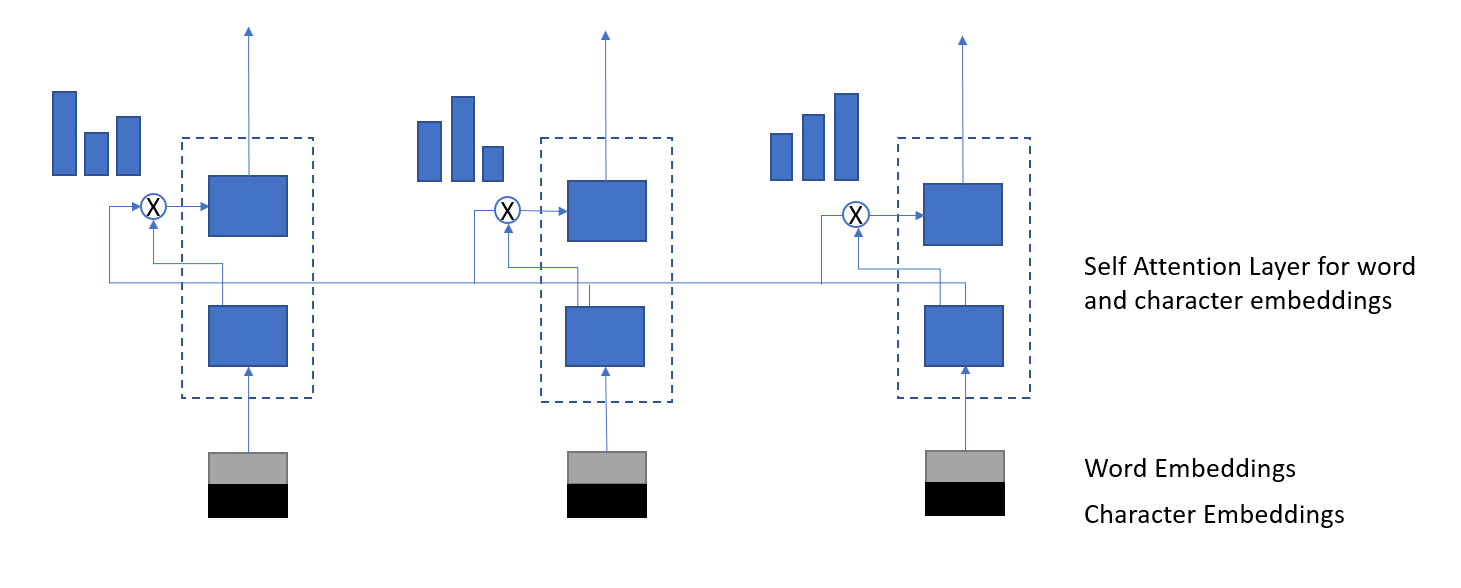
\includegraphics[width=12cm]{Figs4Paper/EarlyAttentionLayer.eps}
  %\caption{Convolutional network architecture}
  %\label{fig:convnetarchitecture}
%\end{figure*}
 
\subsection{Model Training and Scoring}
\label{subsec:modeltrainingandscoring}

\paragraph{Training.} We define the training loss as the sum of the negative log-likelihood (cross-entropy) loss for the start and end locations. So for a (context, question) pair with \textit{start} index {i} $\in \{1, 2, ..., T\}$ and \textit{end} index {j} $\in \{1, 2, ..., T\}$

\begin{equation}
\text{loss} = - \text{log} \, \bm{p}_{start}(i) - \text{log} \, \bm{p}_{end}(j).
\end{equation}

During training, we average across the batch and use the Adadelta optimizer \cite{zeiler2012adadelta} to minimize the loss.

\paragraph{Scoring.} At test time, we chose the pair (i,j) of indices that maximizes $\bm{p}_{start}(i).\bm{p}_{end}(j)$ subject to $i \leq j$ and $j - i + 1 \leq L_{max}$, where $L_{max}$ is a hyperparameter which sets the maximum length of a predicted answer.  

\paragraph{No Answer.}  We adopt the approach proposed by Levy et al \cite{levy2017zero}. We prepend a OOV token to the beginning of each sequence. The model outputs $\bm{p}_{start}$ and $\bm{p}_{end}$ soft-predictions as usual. When discretizing a prediction, if $\bm{p}_{start}(0)$· $\bm{p}_{end}(0)$ is greater than any predicted answer span, the model predicts no-answer. Otherwise the model predicts the highest probability span. Note, this approach also allows us to predict a per-example confidence score that the question is unanswerable.